\chapter{第4章予定地\label{c4}}
\begin{comment}
機械学習
評価指標
など
\end{comment}

\section{4.1\label{c4s1}}
機械学習の分野には,自然言語処理がある.自然言語とは人間が日常的に使用している言語を指し,これをコンピュータを用いて処理する技術のことである.自然言語処理には大きく4つの段階でテキストデータの処理を行う.

\begin{enumerate}
    \item 形態素解析
    \item 構文解析
    \item 意味解析
    \item 文脈解析
\end{enumerate}

自然言語処理を行う上で,処理の対象となる文書データと,文書に含まれる単語を識別するための辞書が必要となる.自然言語処理分野において課題に挙げられることは,自然言語が本質的に持つ「曖昧さ」が挙げられ,これが文章の解釈が複雑になる要因となっている.これは,単語が持つ意味が複数存在し,その単語が用いられている文章の文脈によって意味が変化するためである.この影響を軽減させるためには,自然言語処理を行うモデルに大量のテキストデータを学習させる必要がある.

\section{二値分類における評価指標 \label{c4s2}}

\subsection{混合行列 \label{c4s2-1}}
機械学習における二値分類の評価指標に,混合行列(Confusion Matrix)がある.二値分類で出力されたクラス分類結果をまとめた行列であり,二値分類タスクを行う機械学習モデルの評価指標として利用される.
 
% 図挿入予定

混合行列左上のTP(True Positive)は,実際のデータが正であるものに対し正と予想されたデータの数である.FP(False Positive)は,実際のデータが正であるものに対し負と予想されたデータである.TN(True Negative)は,実際のデータが負であるものに対し負と予想されたデータである.FN(False Negative)は,実際のデータが負であるものに対し正と予想されたデータの個数である.これら4つの値を用いて,後述する正解率,再現率,適合率,F1値を算出する.

\subsubsection{正解率 \label{c4s2-1a}}
正解率(Accuracy)は,二値分類タスクの評価指標の一つであり,全体の分類結果のうち正答した割合を示す値である.正解率の定義を次式に示す.

$$
Accuracy = \frac{TP+FN}{TP+TN+FP+FN}
$$


\subsubsection{適合率 \label{c4s2-1b}}
適合率は(Precision)は,二値分類タスクにおける評価指標の一つであり,学習モデルが正と予測したもののうち,実際に正であものの割合を示す値である.適合率の定義を次式に示す.

$$
Precision = \frac{TP}{TP+FP}
$$


\subsubsection{再現率 \label{c4s2-1c}}
再現率(Recall)は,二値分類タスクの評価指標の一つれあり,実際のデータに含まれる正クラス全体のうち,学習モデルが正と予測したものの割合を示す値である.再現率の定義を次式に示す.

$$
Recall = \frac{TP}{TP+FN}
$$

\subsubsection{F1値 (F1-score, F-measure) \label{c4s2-1d}}
F1値は,二値分類タスクの一つであり,適合率と再現率の調和平均で算出される値である.適合率と再現率の関係はトレードオフの関係であるため,適合率と再現率の間に差が生じる場合がある.この場合,精度が良いとは一概には判断できない.そのため,これら2つの調和平均を算出し,精度に対し2値のバランスを判断するために用いられる.

$$
F1 = \frac{2 \times Recall \times Precision}{Recall+Precision}
$$


\section{Attention \label{c4s3}}
Attentionは、

\section{Transformer \label{c4s4}}


\section{BERT \label{c4s5}}
\subsection{概要}
BERT とは,Bidirectional Encoder Representations from Transformers の略で, 「Transformerによる双方向のエンコード表現」と訳され,2018 年 10 月に Google の Jacob Devlin らの論文[6] で発表された自然言語処理モデルである.
また,質問応答 (Question Answering) や自然言語推論 (Multi Natural Language Inference) などの 11 種の自然言語処理タスクにおいて当時の最高性能を達成している手法であり,これ以降,このモデルから派生して作られたモデルが多数存在する.
また,現在の Google の検索エンジンにも用いられている.
BERT の学習は,大きく2段階に分けられる.
1つ目がラベル付けされていないデータを学習させる「事前学習」であり,2つ目が事前学習時と比較的少量のデータを用いる「Fine Tuning」である.
事前学習で汎用的なモデルを作成し,Fine Tuningを行うことで,個々のタスクに適応したモデルを作成する.

\subsection{アーキテクチャ}
BERTのモデルアーキテクチャは,双方向のtransformerのエンコーダとなっている.
図aaaにBERTと,BERTと同様に事前学習を利用する自然言語処理モデルを比較したものを示す.

% %\begin{figure}[H]
% 	\centering
% % 	\includegraphics[width=150mm]{image/architechture.png}
% 	\caption{各モデルの構造}
% 	\label{architechture}
% \end{figure}

\subsubsection{Transformers}
Transformer とは,再帰型ニューラルネットワーク (以下,RNN) を一切使わずに Attention のみを使うことで,入力と出力の文章同士の広範囲な依存関係を捉えられるモデルである.[7]
RNN は,単語が連続し順序が重要となるような時系列情報を扱うのに最適であるが,逐次的に処理を行うため,処理に多くの時間を必要とする.
また,離れた位置にある文,単語の依存関係をとらえることが難しいといった問題がある.
Transformerは以上のような問題点を克服したモデルである.
Transformerの構造を図aaaに示す.

% \begin{figure}[H]%3.3
% % 	\centering
% 	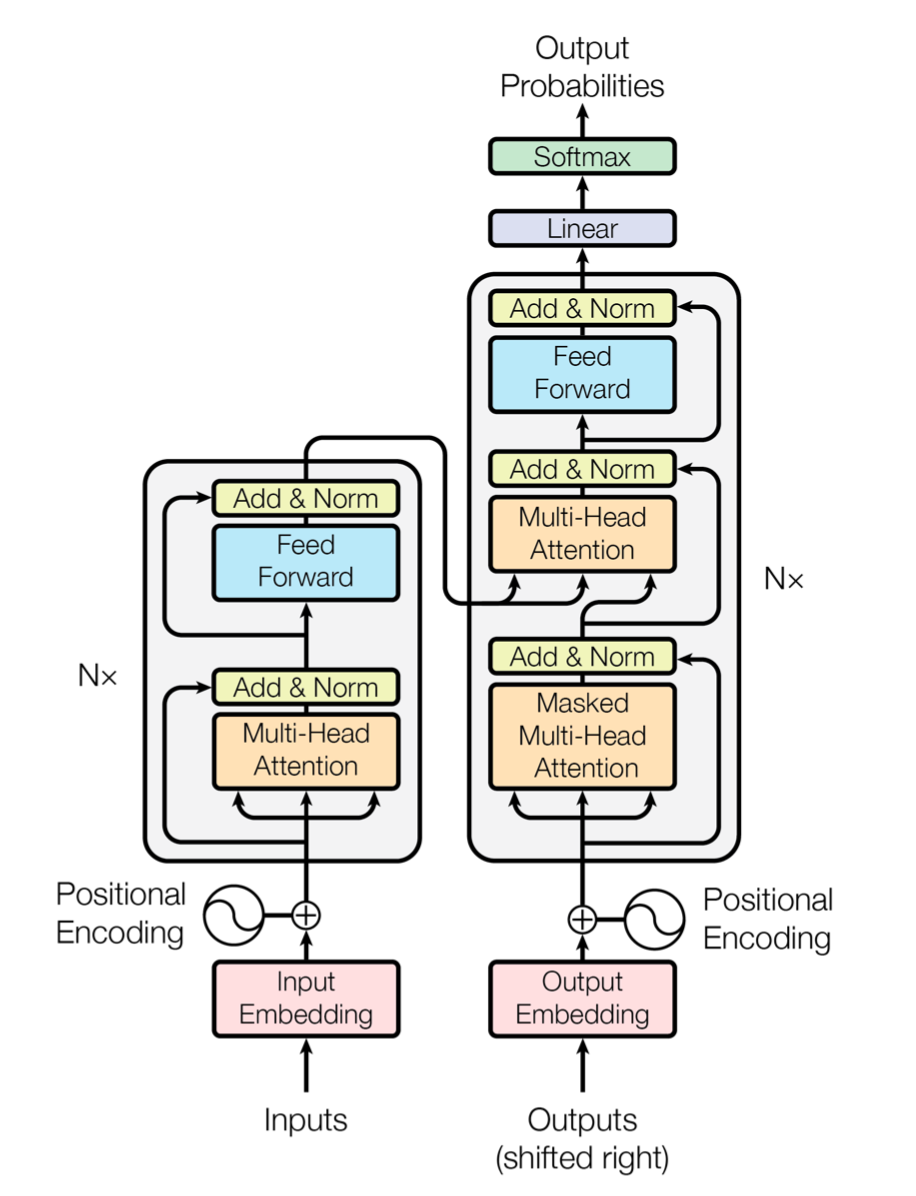
\includegraphics[width=90mm]{image/transformer.png}
% 	\caption{Transformerの構造}
% 	\label{transformer}
% \end{figure}

\subsubsection{Attention}
Attention とは,先述の通り,Transformer の中枢を担う仕組みである.
自然言語処理においては,単語の意味を理解するために,文中のどの単語に注目するすべきかを示すスコアである.Query:${Q}$,Key:${K}$,Value:${V}$の3つのベクトルから計算される.
${K}$と${V}$は1対1の組である.
Attentionは,Self-AttentionとSource-Target-Attentionの2種類がある.また,Attentionの算出方法は加法を使う場合と内積を使う場合があるが,Transformerで使うAttentionは内積を使って算出するため,以降のAttentionの計算は内積を使用していることを前提とする.

\begin{itemize}
	\item Self-Attention \par
	${Q}$, ${K}$, ${V}$は全て同じデータから得られた値を使用する.
	例として「私/は/大学生/です」という文から${Q}$を得たとすると,${K}$, ${V}$も同じ文から取得する.Transformer では Encoder, Decoder の両方に採用され,文の構造や,形態素同士の関係(例文では「私」=「大学生」)を獲得するために使用される.

	\item Target-Attention \par
	${Q}$と${K}$, ${V}$は異なるデータから得られた値を使用する(${K}$, ${V}$は同じデータから取得する).
	例として「風邪/を/引いた」,「病院/に/行く」という2文があるとき,${Q}$は「風邪/を/引いた」から,${K}$, ${V}$は「病院/に/行く」から取得する.
	 Transfomer では Decoder で採用され,「風邪/を/引いた」→「病院/に/行く」という対話の学習に用いられる.
	入力文に対応する出力文が出力されるように学習を行う.
\end{itemize}

以上の Attention を基本とし,Transformers では Scaled Dot-Product Attention と Multi-Head Attentionが実装されている.
その仕組みを図aaa,図aaaに示す.

% % \begin{figure}[H]
% 	\centering
% 	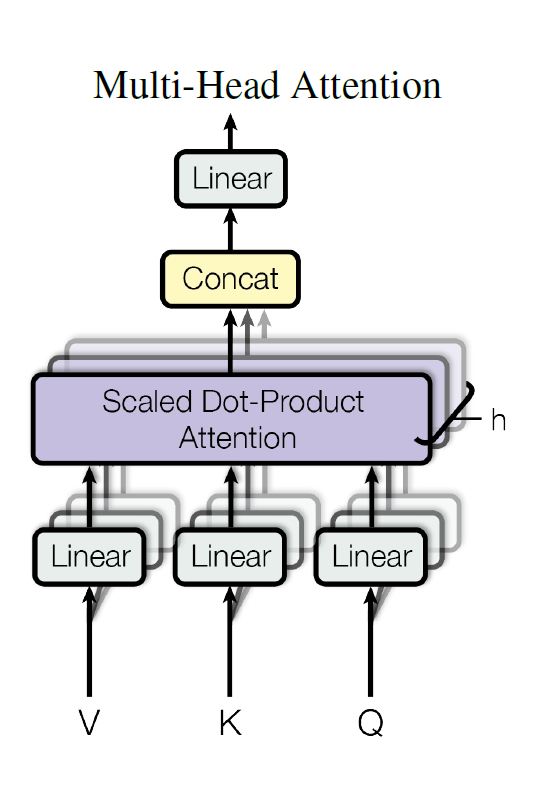
\includegraphics[width=80mm]{image/transformer-multi-head-attention.png}
% 	\caption{Multi-Head Attentionの構造}
% 	\label{mha}
% \end{figure}

% % \begin{figure}[H]
% 	\centering
% 	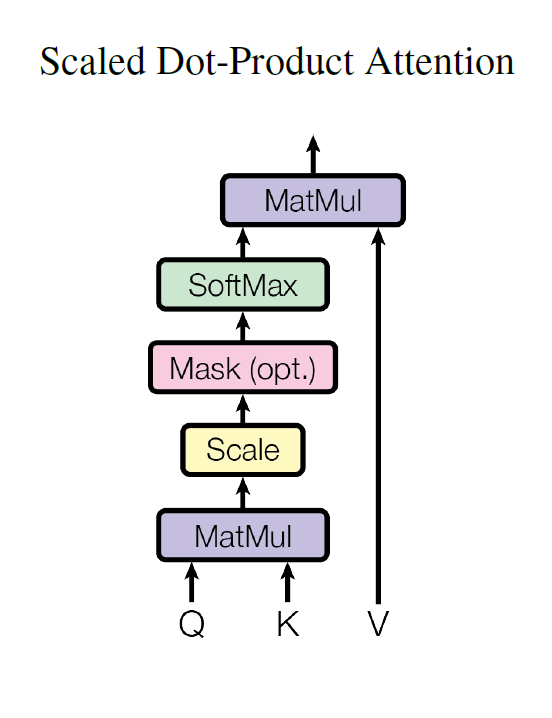
\includegraphics[width=80mm]{image/transformer-scaled-dot-product-attention.png}
% 	\caption{Scaled Dot-Product Attentionの構造}
% 	\label{sda}
% \end{figure}

% 	${Q}$ ${K}$ ${V}$

\begin{itemize}
\item Scaled Dot-Product Attention \par
\par ${Q}$に対応する${K}$を探し,その${K}$を元にして対応する${V}$を取得する.
まず,${Q}$と${K}$の内積${QK^T}$を取ることで${Q}$に対する${K}$の関連度を算出する.
次に softmax 関数を用いて正規化する.ここで,正規化された値は,Attention の重みであり${Q}$に対応する${K}$の位置を示している.
次に Attention の重みと${V}$の内積を求め,${K}$の位置に対応する${V}$を加重和として取得する.
図 3.5 の数式を式(\ref{attention})に,softmax 関数を式(\ref{softmax})に示す.

\begin{equation}
    \mbox{Attention}(Q,K,V) = \mbox{softmax}\left( \frac{QK^T}{\sqrt{d_k}}\right)
    \label{attention}
\end{equation}

\begin{equation}
    \label{softmax}
    \frac{\exp(a_i)}{\sum_{j=1}^{n}\exp(a_j)} \quad(i=1,...,n)
\end{equation}

${QK^T}$の値は次元数に比例して大きくなり,勾配は小さくなってしまう.
そこで式\ref{attention}では${QK^T}$を${\sqrt{d_k}}$で割ることで${QK^T}$の値の増大を防いでいる.
ここで,${d_k}$は${Q}$の次元数を後述する Multi-Head Attention の Head 数で割った値である.

\begin{equation}
    \label{dk}
    d_k = \frac{Q\mbox{の次元数}}{\mbox{Multi-Head Attention のHead数}}
\end{equation}

\item Multi-Head Attention \par
Multi-Head Attention は,Scaled Dot-Product Attention を1つの Head として,複数の Head を並列で処理する仕組みである.
仮に,Head 数が 8 , ${Q}$, ${K}$, ${V}$ の次元数が 512 とすると${\frac{512}{8}=64}$であり,次元数が 64 の ${Q}$, ${K}$, ${V}$ を用いた Scaled Dot-Product Attention を並列に 8 個処理することになる.最終的には個別に計算された値を 1 つのベクトルに落とし込む(concat)ことで単語の分散表現を得る.
この Multi-Head Attention を 1 つのユニット(図 3.2 の Trm )として全結合的に接続したものが BERT モデルである.

\end{itemize}

\section{LLM \label{c4s6}}
LLMとは、Large Language Model の略称であり、大規模言語モデルと呼ばれる。大規模言語モデルという用語についての正式な定義はないが、大規模コーパスを用いて事前学習を行っており、パラメータ総数が数百万以上の言語モデルを指して言われることが多い。LLMの例として、先述のBERTやOpenAI社が開発したGPT-3が挙げられる。

